\documentclass[10pt]{beamer}
\usetheme{metropolis}
% all imports
\usepackage[utf8]{inputenc}
\usepackage[T1]{fontenc}
\usepackage{lmodern}
\usepackage{amsmath}
\usepackage{hyperref}
\usepackage{booktabs}
\usepackage{bm}
\usepackage[scale=2]{ccicons}
\usepackage[outputdir=build]{minted}
\usepackage{pgfplots}
\usepackage{array,colortbl,xcolor}
\usepgfplotslibrary{dateplot}
\usepackage{setspace}
\usepackage{etoolbox}
\usepackage{xspace}
\usepackage{tikz}
\usetikzlibrary{shapes,arrows,positioning,fit,backgrounds}
\usepackage{tkz-euclide}

\AtBeginEnvironment{quote}{\singlespacing}

\AtBeginEnvironment{quote}{\singlespacing}

% new commands
\newcommand{\vect}[1]{\bm{#1}}
\newcommand{\myprime}[1]{{#1}^{\prime}}
\newcommand{\grad}[2]{\nabla_{#1} {#2}}
\newcommand{\dotp}[2]{{#1}^{\top}{#2}}
\newcommand{\dotpPright}[2]{{#1}^{\top}\left({#2}\right)}
\newcommand{\outerp}[2]{\left({#1}\right){#2}^{\top}}
\newcommand{\Jacobian}[2]{\frac{\partial #1}{\partial #2}}
\newcommand{\Vocab}{\mathbb{V}}
 \DeclareMathOperator*{\argmin}{arg\,min}
 \DeclareMathOperator{\E}{\mathbb{E}}

% definitions
\definecolor{blue}{RGB}{159, 192, 176}
\definecolor{green}{RGB}{160, 227, 127}
\definecolor{orange}{RGB}{243, 188, 125}
\definecolor{red}{RGB}{253, 123, 84}
\definecolor{nephritis}{RGB}{39, 174, 96}
\definecolor{emerald}{RGB}{46, 204, 113}
\definecolor{turquoise}{RGB}{39, 174, 96}
\definecolor{green-sea}{RGB}{22, 160, 133}
\definecolor{purple}{RGB}{181, 124, 215}
% Tikzstyles for Computation Graphs

% nodes
\tikzstyle{noop} = [circle, draw=none, fill=red, minimum size = 10pt]
\tikzstyle{op} = [circle, draw=red, line width=1.5pt, fill=red!70, text=black, text centered, font=\bf \normalsize, minimum size = 25pt]
\tikzstyle{op2} = [circle, draw=orange, line width=1.5pt, fill=orange!70, text=black, text centered, font=\bf \normalsize, minimum size = 25pt]
\tikzstyle{op3} = [circle, draw=orange, line width=1.5pt, fill=orange!70, text=black, text centered, font=\bf \scriptsize, minimum size = 7pt]
\tikzstyle{placeholder} = [circle, draw=red, line width=1.5pt, fill=red!30, text=black, text centered, font=\bf  \normalsize, minimum size = 25pt]
\tikzstyle{state} = [circle, draw=blue, line width=1.5pt, fill=blue!70, text=black, text centered, font=\bf \normalsize, minimum size = 25pt]
\tikzstyle{gradient} = [circle, draw=nephritis, line width=1.5pt, fill=nephritis!60, text=black, text centered, font=\bf \normalsize, minimum size = 25pt]
\tikzstyle{gradient2} = [circle, draw=green2, line width=1.5pt, fill=green2!60, text=black, text centered, font=\bf \normalsize, minimum size = 25pt]
\tikzstyle{textonly} = [draw=none, fill=none, text centered, font=\bf \normalsize]

% edges
% \tikzstyle{tedge}  = [draw, thick, >=stealth, ->]
\tikzstyle{tedge}  = [draw, thick, >=latex, ->]
\tikzstyle{tedge_dashed}  = [draw, thick, >=latex, ->, dashed]

% namedscope
\tikzstyle{namedscope} = [circle, draw=orange, line width=1.5pt, fill=orange!60, align=center, inner sep=0pt]

% \tikzstyle{container} = [draw=none, rectangle, dotted, inner ysep=1.5em]
% \tikzstyle{novertex} = [draw=none, fill=none, text centered]
% \tikzstyle{predicate} = [ellipse, draw, thick, text centered, rounded corners, minimum size=30pt]
% \tikzstyle{aux} = [rectangle, draw, thick, text centered, rounded corners, minimum size=30pt]
% \tikzstyle{ledge}  = [draw, dashed, thick, >=stealth, ->]
% \tikzstyle{pedge}  = [draw, thick, >=stealth, ->]


\title{Adding semantic robustness\\ to dialog agents}
\date{\today}

\vspace{1.1 cm}


\author{
  Felipe Salvatore\\
  \url{https://felipessalvatore.github.io/}
  \vspace{1.1 cm}}

\institute{\textbf{IME-USP}: Instituto de Matemática e Estatística - Universidade de São Paulo}


\begin{document}


\maketitle


\begin{frame}{Problema de pesquisa}
falar do que vou pesquisar
\end{frame}


% \begin{frame}{Sistemas de diálogo}
% \begin{itemize}
% \item \alert{Goal-driven systems}:
% \begin{itemize}
% \item serviços de suporte técnico
% \item marketing      
% \item sistemas de reserva
% \item sistemas de informação
% \end{itemize}

% \vspace{0.4cm}
% \item \alert{Non-goal-driven systems}
% \begin{itemize}
% \item Conversas livres (sem fim específico)
% \end{itemize}
% \end{itemize}
% \end{frame}

\section{Background}

\begin{frame}{Neural network based language model}
We call \alert{language model} a probability distribution over sequences of tokens in a natural language.
\begin{equation}
P(x_1,x_2,x_3,x_4) = p
\end{equation}

Since \cite{Mikolov11}, we can use a \alert{Recurrent Neural Network (RNN)} to estimate the probability distribution   \\

\begin{equation}
P(x_{n} = \text{word}_{j^{*}} | x_{1}, \dots ,x_{n-1})
\end{equation}

for any $(n-1)$-sequence of words $x_{1}, \dots ,x_{n-1}$.
\end{frame}

\begin{frame}{Neural network based language model}
% RNN STATE CELL ====================================
\newcommand{\rnnSimpleU}[4]{

% operations
\node[state, minimum size=40pt,#4] (h#3) {$\vect{h}^{#1}$};
\node[op, minimum size=40pt, above=30pt of h#3] (yhat#3){$\hat{\vect{y}}^{#1}$};
\node[op, minimum size=40pt,below=30pt of h#3] (e#3) {$\vect{e}^{#1}$};
\node[textonly, below=0.1pt of e#3] {{\Large#2}};

% edges
\path[tedge] (e#3) edge node[below right= -4pt] {$\vect{U}$} (h#3);
\path[tedge] (h#3) edge node[below right = -4pt] {$\vect{V}$} (yhat#3);
}

\begin{figure}[ht!]
\hspace*{-1.0cm}
\scalebox{0.8}{
\begin{tikzpicture}[auto]

% timestep 1
\rnnSimpleU{(1)}{Yes}{t1}{}

% % timestep 0
\node[state, minimum size=40pt,left=50pt of ht1] (ht0) {$\vect{h}^{(0)}$};

% % timestep 2
\rnnSimpleU{(2)}{here}{t2}{right=50pt of ht1};


% % timestep 2
\rnnSimpleU{(3)}{we}{t3}{right=50pt of ht2};


% % state transfers
\path[tedge] (ht0) edge node[above right = 2pt] {$\vect{W}$} (ht1);
\path[tedge] (ht1) edge node[above right = 2pt] {$\vect{W}$} (ht2);
\path[tedge] (ht2) edge node[above right = 2pt] {$\vect{W}$} (ht3);

% % text
\node[textonly, above=40pt of yhatt2] (result) {{\Large $P(x^{(4)}| \text{Yes, here, we})$}};

% Arrow to result
\draw[->, line width=1mm] [bend right, out=-50, distance=25pt](yhatt3.north) to  (result.east);


\end{tikzpicture}
}%\scalebox
\end{figure}


\end{frame}



\begin{frame}{GRU: Gated Recurrent Units}
\begin{equation}
\vect{\widetilde{h}}^{(t)} = tahn(\vect{W} (\vect{h}^{(t-1)} \odot  \vect{r}^{(t)}) + \vect{U} \vect{x}^{(t)} + \vect{b})
\end{equation}

where $\vect{r}^{(t)}$ is a vector with values in $[0, 1]$ called a \textit{reset gate}, i.e.,  a vector that at each entry outputs the probability of reseting the  corresponding entry in the previous hidden state $\vect{h}^{(t-1)}$. Together with $\vect{r}^{(t)}$ we define an \textit{update gate}, $\vect{u}^{(t)}$. It is also a vector with values in $[0, 1]$. Intuitively we can say that this vector decides how much on each dimension we will use the candidate update. Both $\vect{r}^{(t)}$ and $\vect{u}^{(t)}$ are defined by $\vect{h}^{(t-1)}$ and $\vect{x}^{(t)}$; they also have specific parameters:

\begin{equation}
\vect{r}^{(t)} = \sigma(\vect{W}_{r} \vect{h}^{(t-1)} + \vect{U}_{r} \vect{x}^{(t)} + \vect{b}_{r})
\end{equation}


\begin{equation}
\vect{u}^{(t)} = \sigma(\vect{W}_{u} \vect{h}^{(t-1)} + \vect{U}_{u} \vect{x}^{(t)} + \vect{b}_{u})
\end{equation}

At the end the new hidden state $\vect{h}^{(t)}$ is defined by the recurrence:

\begin{equation}
\vect{h}^{(t)} = \vect{u}^{(t)} \odot \vect{\widetilde{h}}^{(t)} + (1 - \vect{u}^{(t)}) \odot \vect{h}^{(t-1)} 
\end{equation}

\end{frame}

\begin{frame}{LSTM: Long Short Term Memory}
\begin{equation}
\vect{f}^{(t)} = \sigma(\vect{W}_{f} \vect{h}^{(t-1)} + \vect{U}_{f} \vect{x}^{(t)} + \vect{b}_{f})
\end{equation}

\begin{equation}
\vect{i}^{(t)} = \sigma(\vect{W}_{i} \vect{h}^{(t-1)} + \vect{U}_{i} \vect{x}^{(t)} + \vect{b}_{i})
\end{equation}

\begin{equation}
\vect{o}^{(t)} = \sigma(\vect{W}_{o} \vect{h}^{(t-1)} + \vect{U}_{o} \vect{x}^{(t)} + \vect{b}_{o})
\end{equation}

Intuitively $\vect{f}^{(t)}$ should control how much informative will be discarded, $\vect{i}^{(t)}$ controls how much information will be updated, and $\vect{o}^{(t)}$ controls how munch each component should be outputted. A candidate cell, $\tilde{\vect{c}}^{(t)}$ is formed:

\begin{equation}
\tilde{\vect{c}}^{(t)} = tahn(\vect{W} \vect{h}^{(t-1)} + \vect{U} \vect{x}^{(t)} + \vect{b})
\end{equation}

And a new cell $\vect{c}^{(t)}$ is formed by forgetting some information of the previous cell $\tilde{\vect{c}}^{(t-1)}$ and by adding new values from $\tilde{\vect{c}}^{(t)}$ (scaled by the input gate)

\begin{equation}
\vect{c}^{(t)} = \vect{f}^{(t)} \odot \vect{c}^{(t-1)} + \vect{i}^{(t)} \odot \tilde{\vect{c}}^{(t)}
\end{equation}
\end{frame}

\begin{frame}{Sequence-to-sequence}
\begin{equation}
\vect{s} = f_{enc}(\vect{x}^{(n)}, \vect{h}^{(n-1)})
\end{equation}

\begin{equation}
\vect{\tilde{h}}^{(t)} = f_{dec}(\vect{y}^{(t)}, \vect{\tilde{h}}^{(t-1)})
\end{equation}

\begin{equation}
p(y_t | y_1, \dots, y_{t-1}, x_1, \dots, x_{n}) = softmax(\vect{W}_{s}  \vect{\tilde{h}}^{(t)} + \vect{b}_s)
\end{equation}


\end{frame}

\begin{frame}{Attention}
We will use this matrix as an alignment matrix, i.e., at the end of the training $\vect{a}_{ts}$ should reflect the probability of the source representation $\vect{h}^{(s)}$ be relevant for the output $\hat{y}^{(t)}$. We define $\vect{a}_{ts}$ as

\begin{equation}
\vect{a}_{ts} = \frac{exp(score(\vect{\tilde{h}}_t,\vect{h}_s))}{\sum_j exp(score(\vect{\tilde{h}}_t,\vect{h}_j))}
\end{equation}

Where $score$ is a content-based function that can have different implementations: 

\begin{equation}
score(\vect{\tilde{h}}_t,\vect{h}_s) = \begin{cases}
\vect{\tilde{h}}_t ^{\top}\vect{h}_s\\
\vect{\tilde{h}}_t ^{\top}\vect{W}_a \vect{h}_s\\
\vect{v}_a ^{\top}tahn(\vect{W}_a[\vect{\tilde{h}}_t;\vect{h}_s])\\
\end{cases}
\end{equation}

At the end, a global context vector $\vect{c}^{(t)}$ is computed as the weighted average, according to $\vect{a}_t$ over all source states:

\begin{equation}
\vect{c}^{(t)} = \sum_{s} \vect{a}_{ts}\vect{h}^{(s)}
\end{equation}


\end{frame}


\section{Neural network based dialog systems}

\begin{frame}{Seq2seq applied to translation}
% RNN encoder ====================================
\newcommand{\rnnencoder}[4]{

% operations
\node[state, minimum size=40pt,#4] (h#3) {$\vect{h}^{#1}$};
\node[op, minimum size=40pt,below=30pt of h#3] (e#3) {$\vect{e}^{#1}$};
\node[textonly, below=0.1pt of e#3] {{\Large#2}};

% edges
\path[tedge] (e#3) edge node[below right= -4pt] {} (h#3);
}

% RNN decoder ====================================
\newcommand{\rnndecoder}[4]{

% operations
\node[state, minimum size=40pt,#4] (h#3) {${\vect{h}^{\prime}}^{#1}$};
\node[output, minimum size=40pt, above=30pt of h#3] (yhat#3){$\hat{\vect{y}}^{#1}$};
\node[op, minimum size=40pt,below=30pt of h#3] (x#3) {$\vect{x}^{#1}$};
\node[textonly, below=0.1pt of x#3] {{\Large#2}};

% edges
\path[tedge] (x#3) edge node[below right= -4pt] {} (h#3);
\path[tedge] (h#3) edge node[below right = -4pt] {} (yhat#3);
}


\newcommand{\rnndecoderSimpl}[4]{

% operations
\node[state, minimum size=40pt,#4] (h#3) {${\vect{h}^{\prime}}^{#1}$};
\node[op, minimum size=40pt,below=30pt of h#3] (x#3) {$\vect{x}^{#1}$};
\node[textonly, below=0.1pt of x#3] {{\Large#2}};

% edges
\path[tedge] (x#3) edge node[below right= -4pt] {} (h#3);
}


\begin{figure}[ht!]
\hspace*{-1.0cm}
\scalebox{0.5}{
\begin{tikzpicture}[auto]

% timestep encoder 1
\rnnencoder{(1)}{What}{t1}{}

% timestep encoder 0
\node[state, minimum size=40pt,left=40pt of ht1] (ht0) {$\vect{h}^{(0)}$};

%  timestep encoder 2
\rnnencoder{(2)}{are}{t2}{right=40pt of ht1};

%  timestep encoder 3
\rnnencoder{(3)}{the}{t3}{right=40pt of ht2};

%  timestep encoder 4
\rnnencoder{(4)}{cities}{t4}{right=40pt of ht3};

%  timestep encoder 5
\rnnencoder{(5)}{of}{t5}{right=40pt of ht4};

%  timestep encoder 6
\rnnencoder{(6)}{Texas}{t6}{right=40pt of ht5};

%  timestep encoder 7
\rnnencoder{(7)}{?}{t7}{right=40pt of ht6};

% % state transfers encoder
\path[tedge] (ht0) -- (ht1);
\path[tedge] (ht1) --  (ht2);
\path[tedge] (ht2) -- (ht3);
\path[tedge] (ht3) -- (ht4);
\path[tedge] (ht4) --  (ht5);
\path[tedge] (ht5) -- (ht6);
\path[tedge] (ht6) -- (ht7);

%  timestep decoder 1
\rnndecoderSimpl{(1)}{SELECT}{tt1}{above=190pt of ht3};

%  timestep decoder 2
\rnndecoderSimpl{(2)}{?city}{tt2}{right=40pt of htt1};

%  timestep decoder 3
\rnndecoderSimpl{(3)}{$\{$}{tt3}{right=40pt of htt2};

%  timestep decoder 4
\rnndecoder{(4)}{?Texas}{tt4}{right=40pt of htt3};


% % state transfers encoder
\path[tedge] (htt1) --  (htt2);
\path[tedge] (htt2) -- (htt3);
\path[tedge] (htt3) -- (htt4);


% text
\node[textonly, left=40pt of yhattt4] (result) {{\Large $P(x^{(5)}| \text{SELECT, ?city, } \{ \text{ , ?Texas, } \vect{h}^{(7)})$}};

% Arrow to result
\draw[->, line width=1mm] (yhattt4) to  (result.east);

% encoder to decoder
\node[state, minimum size=40pt, above=70pt of ht1] (2ht7) {$\vect{h}^{(7)}$};


% bent Arrow
\path[tedge] (ht7) edge [out=120, in=-20] node {} (2ht7);
\path[tedge] (2ht7) edge [out=90, in=180] node {} (htt1);




\end{tikzpicture}
}%\scalebox
\end{figure}


\end{frame}

\begin{frame}{Seq2seq applied to dialog \cite{DBLP:journals/corr/VinyalsL15}}
% RNN encoder ====================================
\newcommand{\rnnencoder}[4]{

% operations
\node[state, minimum size=40pt,#4] (h#3) {$\vect{h}^{#1}$};
\node[op, minimum size=40pt,below=30pt of h#3] (e#3) {$\vect{e}^{#1}$};
\node[textonly, below=0.1pt of e#3] {{\Large#2}};

% edges
\path[tedge] (e#3) edge node[below right= -4pt] {} (h#3);
}

% RNN decoder ====================================
\newcommand{\rnndecoder}[4]{

% operations
\node[state, minimum size=40pt,#4] (h#3) {${\vect{h}^{\prime}}^{#1}$};
\node[output, minimum size=40pt, above=30pt of h#3] (yhat#3){$\hat{\vect{y}}^{#1}$};
\node[op, minimum size=40pt,below=30pt of h#3] (x#3) {$\vect{x}^{#1}$};
\node[textonly, below=0.1pt of x#3] {{\Large#2}};

% edges
\path[tedge] (x#3) edge node[below right= -4pt] {} (h#3);
\path[tedge] (h#3) edge node[below right = -4pt] {} (yhat#3);
}


\newcommand{\rnndecoderSimpl}[4]{

% operations
\node[state, minimum size=40pt,#4] (h#3) {${\vect{h}^{\prime}}^{#1}$};
\node[op, minimum size=40pt,below=30pt of h#3] (x#3) {$\vect{x}^{#1}$};
\node[textonly, below=0.1pt of x#3] {{\Large#2}};

% edges
\path[tedge] (x#3) edge node[below right= -4pt] {} (h#3);
}


\begin{figure}[ht!]
\hspace*{-1.0cm}
\scalebox{0.5}{
\begin{tikzpicture}[auto]

% timestep encoder 1
\rnnencoder{(1)}{What}{t1}{}

% timestep encoder 0
\node[state, minimum size=40pt,left=40pt of ht1] (ht0) {$\vect{h}^{(0)}$};

%  timestep encoder 2
\rnnencoder{(2)}{are}{t2}{right=40pt of ht1};

%  timestep encoder 3
\rnnencoder{(3)}{you}{t3}{right=40pt of ht2};

%  timestep encoder 4
\rnnencoder{(4)}{doing}{t4}{right=40pt of ht3};

%  timestep encoder 5
\rnnencoder{(5)}{right}{t5}{right=40pt of ht4};

%  timestep encoder 6
\rnnencoder{(6)}{now}{t6}{right=40pt of ht5};

%  timestep encoder 7
\rnnencoder{(7)}{?}{t7}{right=40pt of ht6};

% % state transfers encoder
\path[tedge] (ht0) -- (ht1);
\path[tedge] (ht1) --  (ht2);
\path[tedge] (ht2) -- (ht3);
\path[tedge] (ht3) -- (ht4);
\path[tedge] (ht4) --  (ht5);
\path[tedge] (ht5) -- (ht6);
\path[tedge] (ht6) -- (ht7);

%  timestep decoder 1
\rnndecoderSimpl{(1)}{I}{tt1}{above=190pt of ht3};

%  timestep decoder 2
\rnndecoderSimpl{(2)}{just}{tt2}{right=40pt of htt1};

%  timestep decoder 3
\rnndecoderSimpl{(3)}{start}{tt3}{right=40pt of htt2};

%  timestep decoder 4
\rnndecoder{(4)}{cleaning}{tt4}{right=40pt of htt3};


% % state transfers encoder
\path[tedge] (htt1) --  (htt2);
\path[tedge] (htt2) -- (htt3);
\path[tedge] (htt3) -- (htt4);


% text
\node[textonly, left=40pt of yhattt4] (result) {{\Large $P(x^{(5)}| \text{I, just, start, cleaning,  }\vect{h}^{(7)})$}};

% Arrow to result
\draw[->, line width=1mm] (yhattt4) to  (result.east);

% encoder to decoder
\node[state, minimum size=40pt, above=70pt of ht1] (2ht7) {$\vect{h}^{(7)}$};


% bent Arrow
\path[tedge] (ht7) edge [out=120, in=-20] node {} (2ht7);
\path[tedge] (2ht7) edge [out=90, in=180] node {} (htt1);




\end{tikzpicture}
}%\scalebox
\end{figure}


\end{frame}


\begin{frame}{Modelo de memória}
\begin{itemize}
\item $\vect{s}_1, \dots, \vect{s}_n$ sentenças de contexto
\item $\vect{q}$ pergunta
\item $\vect{a}$ resposta
\item $\{ \vect{s}_i\} \rightarrow^{\vect{A}} \{ \vect{m}_i\}$  (vetores de memôria)
\item $\vect{q} \rightarrow^{\vect{B}} \vect{u}$  (estado interno)
\item $\{ p_i\} = \{ softmax(\vect{u}^{T}\vect{m}_i)\}$  ("match" entre $\vect{m}_i$ e $\vect{u}$)
\item $\{ \vect{s}_i\} \rightarrow^{\vect{C}} \{ \vect{c}_i\}$
\item $\vect{o}= \sum_{i} p_i \vect{c}_i$
\item $\vect{\hat{a}}= softmax(\vect{W}(\vect{o} + \vect{u}))$
\end{itemize}
\end{frame}


\begin{frame}{ Podemos ter $k$ camadas e memória (hops)}
\begin{itemize}
\item $\vect{u}^{k} = \vect{u}^{k-1} + \vect{o}^{k-1}$
\item[]
\item $\{ {\vect{s}^{k}}_i\} \rightarrow^{{vect{A}^{k}}} \{ {\vect{m}^{k}}_i\}$
\item[]
\item $\{ {\vect{s}^{k}}_i\} \rightarrow^{{vect{C}^{k}}} \{ {\vect{c}^{k}}_i\}$
\item[]
\item $\{{p^{k}}_i\} = \{ softmax({\vect{u}^{k}}^{\top} {\vect{m}^{k}_{i}})\}$
\item[]
\item $\vect{o}^{k}= \sum_{i} {p^{k}}_i {\vect{c}^{k}}_i$
\item[]
\item $\vect{\hat{a}}= softmax(\vect{W}(\vect{o}^{k} + \vect{u}^{k}))$
\end{itemize}
\end{frame}

\begin{frame}{MemNN}
The memory model is defined by $k$ memory layers, each layer is compose of the following parts:


\begin{itemize}
\item $\{ {\vect{m}^{k}}_i\}$ is an $n$-sequence of \textit{memory vectors}. Where $i = 1, \dots, n$ and $\vect{m}^{k}_i = \sum_{j} \vect{A}^{k}x_{i,j}$.
\item  $\vect{u}^{k}$ is the \textit{input vector}, where
\begin{equation}
\vect{u}^{k}=
\begin{cases}
\sum_{j} \vect{B}^{k}w_{j} & \text{if } k=1, \\
\vect{u}^{k-1} + \vect{o}^{k-1}  & \text{otherwise}\\
\end{cases}
\end{equation}
\item $\vect{p}^{k} \in \mathbb{R}^{n}$ is the \textit{match between the input vector} $\vect{u}^{k}$ \textit{and each memory vector} ${\vect{m}^{k}}_i$. $\vect{p}^{k}$ is defined as
\begin{equation}
{\vect{p}^{k}}_i = softmax({\vect{u}^{k}}^{\top} {\vect{m}^{k}}_i) 
\end{equation}
\item $\{ {\vect{c}^{k}}_i\}$ is another representation of the context $U_1, ..., U_n$ defined by another embedding matrix $\vect{C}$, i.e., $\vect{c}^{k}_i = \sum_{j} \vect{C}^{k}x_{i,j}$.
\item $\vect{o}^{k}$ is the memory layer's  \textit{output}. It is a sum over the transformed context $\{ {\vect{c}^{k}}_i\}$ weighted by the probability vector $\vect{p}^{k}$ defined by the input $\vect{u}^{k}$, i.e.,  $\vect{o}^{k}= \sum_{i} {\vect{p}^{k}}_i {\vect{c}^{k}}_i$.
\end{itemize}

Note that each memory layer $k$ is defined by three embedding matrices $\vect{A}^{k}, \vect{B}^{k}, \vect{C}^{k} \in \mathbb{R}^{d,V}$ where $d$, the size of the embedding, is a hyperparameter.

After all the $K$ memory layers have computed their output, the model's prediction is a probability distribution over all the tokens in the vocabulary, remember here the answer is composed of one word only:
\begin{equation}
\vect{\hat{a}}= softmax(\vect{W}(\vect{o}^{K}))
\end{equation}

\end{frame}



\section{How to evaluate dialogs?}


\begin{frame}{Human evaluation  \cite{Lowe:2016}}
\begin{center}
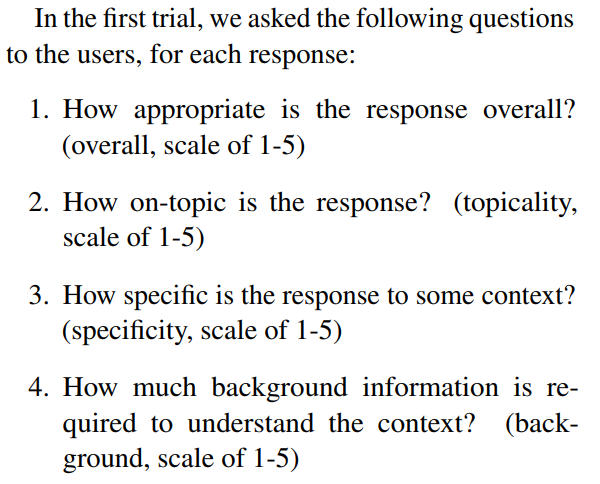
\includegraphics[scale=0.2]{images/exemploEval1.png}
\end{center}

\begin{enumerate}
\item \alert{Adequacy}: the meaning equivalence between the generated and control sentence. 
\item \alert{Fluency}: the syntactic correctness of the generated sequence.
\item \alert{Readability}: efficacy of the generated sentence in a particular context.
\end{enumerate}

\end{frame}

\begin{frame}{BLEU (bilingual evaluation understudy) \cite{Papineni2001}}
\begin{equation}
P_n = \frac{\text{number of } n\text{-grams in both } \hat{y} \text{ and } y}{\text{number of } n\text{-grams appearing in } \hat{y}}
\end{equation}    
\vspace{0.2cm}

\begin{equation}
BP=
\begin{cases}
1 & \text{if } len(\hat{y}) > len(y) \\
\exp\left( 1 - \frac{len(y)}{len(\hat{y})} \right) & \text{otherwise}
\end{cases}
\end{equation} 
\vspace{0.2cm}

\begin{equation}
BLEU = BP \; \exp \left(\frac{1}{N}  \sum_{n=1}^{N} \log P_n \right)
\end{equation}
\end{frame}


\begin{frame}{METEOR (Metric for Evaluation of Translation with Explicit ORdering) \cite{Lavie}}
\begin{equation}
P = \frac{\text{number of } \text{unigrams in both } \hat{y} \text{ and } y}{\text{number of } \text{unigrams appearing in } \hat{y}}
\end{equation}    


\begin{equation}
R = \frac{\text{number of } \text{unigrams in both } \hat{y} \text{ and } y}{\text{number of } \text{unigrams appearing in } y}
\end{equation}    


\begin{equation}
F_{mean} = \frac{10 P R}{R + 9P}
\end{equation}

\begin{equation}
METEOR = F_{mean} (1 - penalty)
\end{equation}
\end{frame}

\begin{frame}{ROUGE (Recall Oriented Understudy for Gisting Evaluation) \cite{Lin}}
\begin{equation}
P_{lcs} = \frac{lcs(\hat{y}, y)}{len(\hat{y})}
\end{equation}    


\begin{equation}
R_{lcs} = \frac{lcs(\hat{y}, y)}{len(y)}
\end{equation}

\begin{equation}
ROUGE_L = \frac{(1 + \beta^2) P_{lcs} R_{lcs}}{R_{lcs} + \beta^{2}P_{lcs}}
\end{equation}

where $\beta$ is usually set to favour recal ($\beta = 1.2$).
\end{frame}


\begin{frame}{Problems \cite{LiuLSNCP16}}

\begin{table}[h]
\centering
\label{hownottable}
\begin{tabular}{|c|c|c|c|c|}
\hline
\cellcolor{blue!50} metric & \cellcolor{blue!50} Spearman & \cellcolor{blue!50} $p$-value & \cellcolor{blue!50} Pearson &  \cellcolor{blue!50} $p$-value \\ \hline
BLEU   & $0.34$   & $< 0.01$  & $0.14$  & $0.17$ \\ \hline
METEOR & $0.19$   & $0.06$    & $0.19$  & $0.05$ \\ \hline
ROUGE  & $0.12$   & $0.22$    & $0.1$   & $0.34$ \\ \hline  
\end{tabular}
\caption{Correlation between automatic metrics and human judgments based on dialog generated on Twitter}
\end{table}

\begin{table}[h]
\centering
\label{hownottable}
\begin{tabular}{|c|c|c|c|c|}
\hline
\cellcolor{blue!50} metric & \cellcolor{blue!50} Spearman & \cellcolor{blue!50} $p$-value & \cellcolor{blue!50} Pearson &  \cellcolor{blue!50} $p$-value \\ \hline
BLEU & $0.12$   & $0.23$    & $0.11$  & $0.26$    \\ \hline
METEOR & $0.06$   & $0.53$    & $0.14$  & $0.16$     \\ \hline
ROUGE & $0.05$   & $0.59$    & $0.06$  & $0.53$    \\ \hline
\end{tabular}
\caption{Correlation between automatic metrics and human judgments based on dialog generated on Ubuntu}
\end{table}
\end{frame}

\section{Creating simplified tasks as tests}

\begin{frame}{bAbI \cite{WestonBCM15}}
One solution is to create a set of QA synthetic tasks to test different capabilities of a dialog agent.


\begin{center}
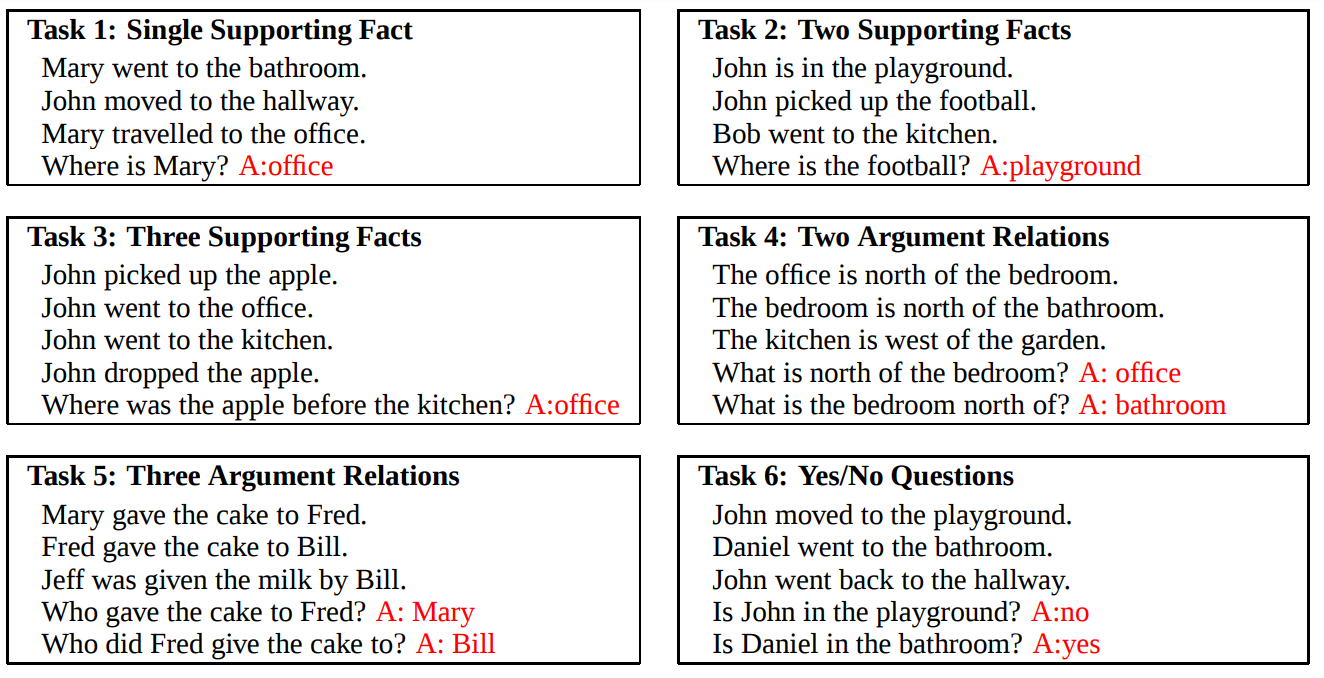
\includegraphics[scale=0.25]{images/babi.png}
\end{center}
\end{frame}



\begin{frame}{ParlAI \\ \url{https://github.com/facebookresearch/ParlAI}}

\begin{center}

\includegraphics[scale=0.84]{images/parlai.png}
\end{center}

"ParlAI (pronounced 'par-lay') is a framework for dialog AI research, implemented in Python.

Its goal is to provide researchers:

\begin{itemize}
\item a unified framework for sharing, training and testing dialog models
\item many popular datasets available all in one place, with the ability to multi-task over them
\item seamless integration of Amazon Mechanical Turk for data collection and human evaluation"
\end{itemize}

\end{frame}

\begin{frame}{Sanity check experiments}
\begin{center}
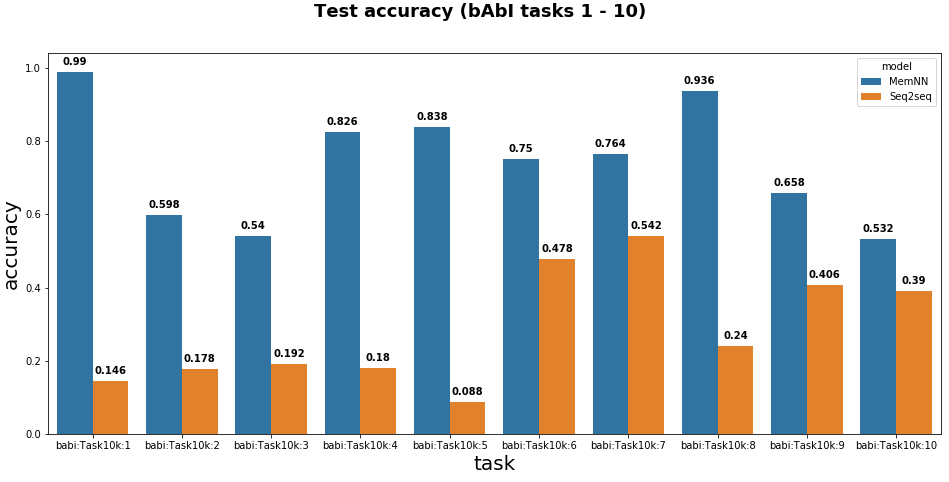
\includegraphics[scale=0.34]{images/comparative_results_babi1.png}
\end{center}
\end{frame}

\begin{frame}{Sanity check experiments}
\begin{center}
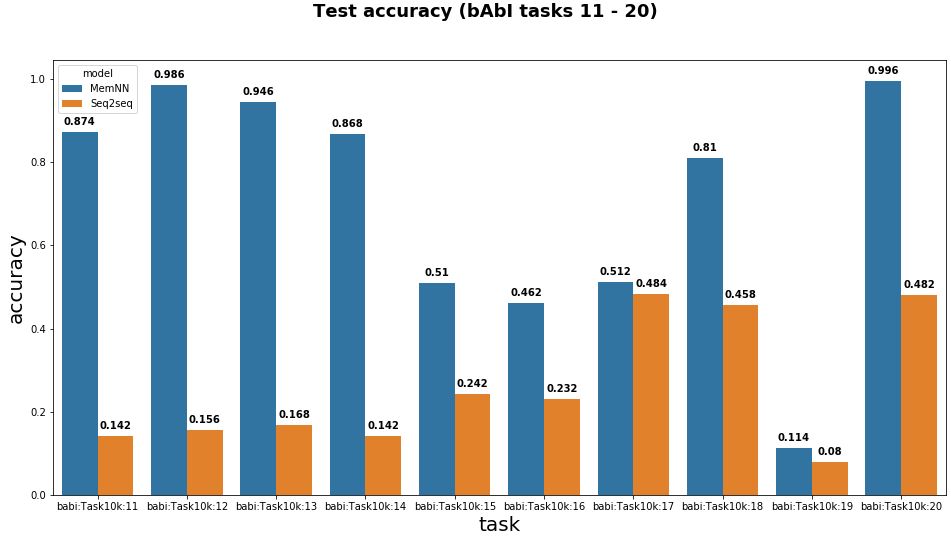
\includegraphics[scale=0.34]{images/comparative_results_babi2.png}
\end{center}
\end{frame}

\section{Entailment-QA}

\begin{frame}{bAbI: task 15}

\alert{Basic Deduction}

\begin{center}
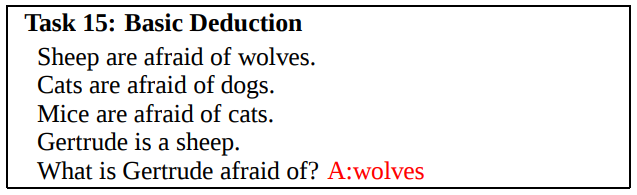
\includegraphics[scale=0.28]{images/babi15.png}
\end{center}
\begin{quote} 
\centering 
$P^{1}$ are afraid of $Q^{1}$\\
$P^{2}$ are afraid of $Q^{2}$\\
$P^{3}$ are afraid of $Q^{3}$\\
$P^{4}$ are afraid of $Q^{4}$\\
$c^{1}$ is a $P^{1}$\\
$c^{2}$ is a $P^{2}$\\
$c^{3}$ is a $P^{3}$\\
$c^{4}$ is a $P^{4}$\\
What is $c^j$ afraid of? \alert{A: $Q^j$}\\
\end{quote}


\end{frame}


\begin{frame}{bAbI: task 16}

\alert{Basic Induction}

\begin{center}
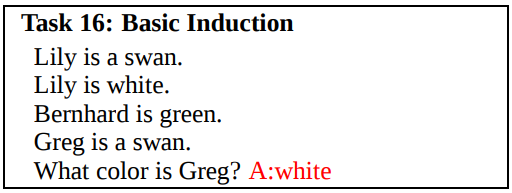
\includegraphics[scale=0.28]{images/babi16.png}
\end{center}
\begin{quote} 
\centering 
$c^{1}$ is a $P^{1}$\\
$c^{1}$ is $C^{1}$\\
$c^{2}$ is a $P^{2}$\\
$c^{2}$ is $C^{2}$\\
$c^{3}$ is a $P^{3}$\\
$c^{3}$ is $C^{3}$\\
$c^{4}$ is a $P^{4}$\\
$c^{4}$ is $C^{4}$\\
$c$ is a $P^{j}$\\
What color is $c$? \alert{A: $C^j$}\\
\end{quote}

\end{frame}




\begin{frame}{Entailment-QA}

\begin{enumerate}
\item \textbf{Boolean Connectives}
\item[]
\item \textbf{First-Order Quantifiers}
\item[]
\item \textbf{Synonymy}
\item[]
\item \textbf{Antinomy}
\item[]
\item \textbf{Hypernymy}
\item[]
\item \textbf{Active/Passive voice}
\end{enumerate}
\end{frame}

\begin{frame}{Entailment-QA: task 1}
\begin{itemize}
\item \alert{Entailment} ($s_1$ implies $s_2$)
\begin{itemize}
\item $\underbrace{P^{1}a^1 \land \dots \land P^{n}a^n}_{s_1}, \underbrace{P^{j}a^j}_{s_2}$ 
\item $\underbrace{P^{j}a^j}_{s_1}, \underbrace{P^{1}a^1 \lor \dots \lor P^{n}a^n}_{s_2}$
\item $\underbrace{Pa}_{s_1}, \underbrace{\lnot \lnot Pa}_{s_2}$
\end{itemize}

\vspace{0.4cm}
\item \alert{Not entailment} ($s_1$ does not imply $s_2$)
\begin{itemize}
\item $\underbrace{P^{j}a^j}_{s_1}, \underbrace{P^{1}a^1 \land \dots \land P^{n}a^n}_{s_2}$ 
\item $\underbrace{P^{1}a^1 \lor \dots \lor P^{n}a^n}_{s_1}, \underbrace{P^{j}a^j}_{s_2}$
\item $\underbrace{Pa}_{s_1}, \underbrace{\lnot Pa}_{s_2}$
\end{itemize}
\end{itemize}
\end{frame}


\begin{frame}{Entailment-QA: task 1}
\begin{itemize} 
\item[] Ashley is fit
\item[] Ashley is not fit
\item[] The first sentence implies the second sentence? \alert{A: no}
\end{itemize}

\vspace{0.3cm}


\begin{itemize} 
\item[]Avery is nice and Avery is obedient
\item[]Avery is nice
\item[]The first sentence implies the second sentence? \alert{A: yes}
\end{itemize}

\vspace{0.3cm}

\begin{itemize} 
\item[]Elbert is handsome or Elbert is long
\item[]Elbert is handsome
\item[]The first sentence implies the second sentence? \alert{A: no}
\end{itemize}
\end{frame}


\begin{frame}{Entailment-QA: task 2}

\begin{itemize}
\item \alert{Entailment}
\begin{itemize}
\item $\forall x Px, Pa$ 
\item $Pa, \exists x Px$ 
\end{itemize}
\item \alert{Contradiction}
\begin{itemize}
\item $\forall x Px, \lnot Pa$ 
\item $\forall x Px, \exists x \lnot Px$ 
\end{itemize}
\item \alert{Neutral}
\begin{itemize}
\item $Pa,Qa$ 
\item $\forall x Px, \lnot Qa$ 
\end{itemize}
\end{itemize}
\end{frame}


\begin{frame}{Entailment-QA: task 2}

\begin{itemize} 
\item[] Every person is lively
\item[] Belden is lively
\item[] What is the semantic relation? \alert{A: entailment}
\end{itemize}

\begin{itemize} 
\item[] Every person is short
\item[] There is one person that is not short
\item[] What is the semantic relation?  \alert{A: contradiction}
\end{itemize}

\begin{itemize} 
\item[] Every person is beautiful
\item[] Abilene is not blue
\item[] What is the semantic relation? \alert{A: neutral}
\end{itemize}
\end{frame}

\begin{frame}{Entailment-QA: task proxy}

SICK (Sentences Involving Compositional Knowledge) \cite{Marelli14}

\begin{center}
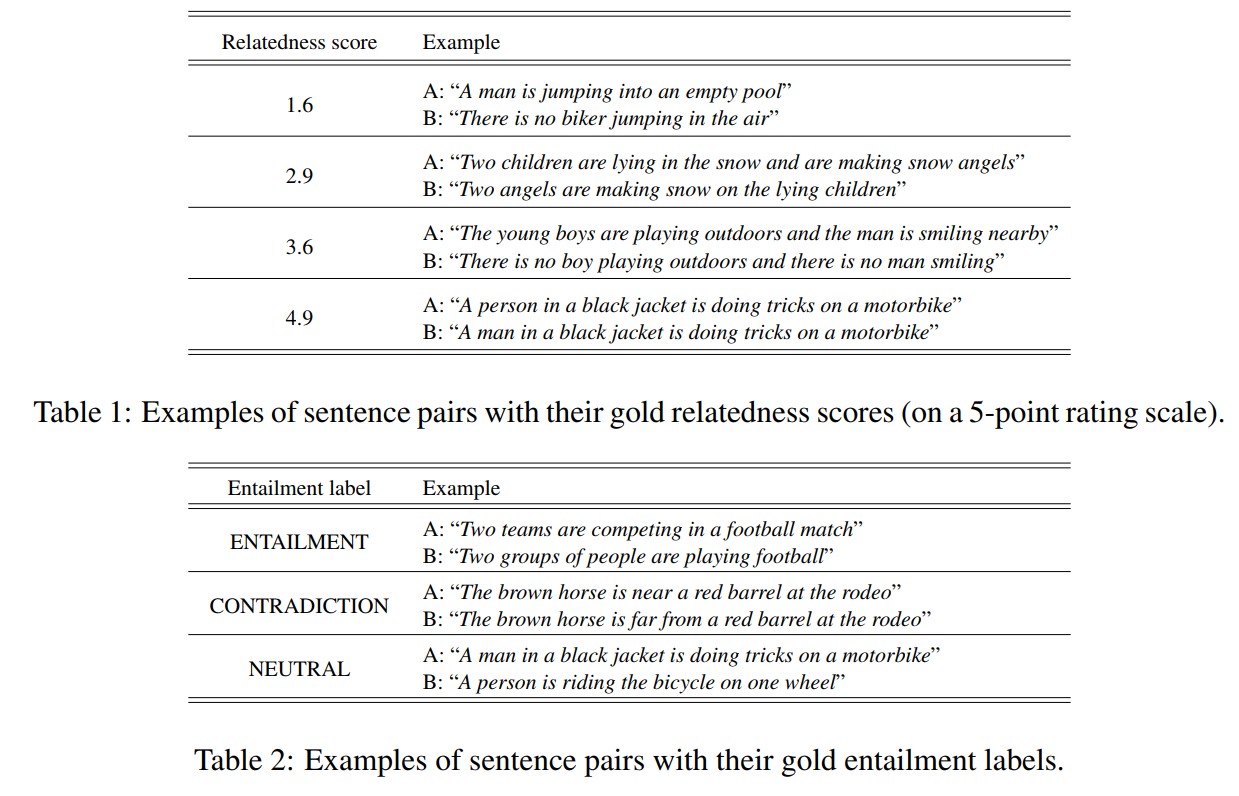
\includegraphics[scale=0.25]{images/sick.png}
\end{center}

\end{frame}


\begin{frame}{Entailment-QA: task proxy}

\begin{itemize} 
\item[] There is no dog leaping in the air
\item[] A dog is leaping high in the air and another is watching
\item[] What is the semantic relation? \alert{A: contradiction}
\end{itemize}

\begin{itemize} 
\item[] A man is exercising
\item[] A baby is laughing
\item[] What is the semantic relation? \alert{A: neutral}
\end{itemize}

\begin{itemize} 
\item[] Some dogs are playing in a river
\item[] Some dogs are playing in a stream
\item[] What is the semantic relation? \alert{A: entailment}
\end{itemize}
\end{frame}



\begin{frame}{Preliminary Results}
\begin{center}
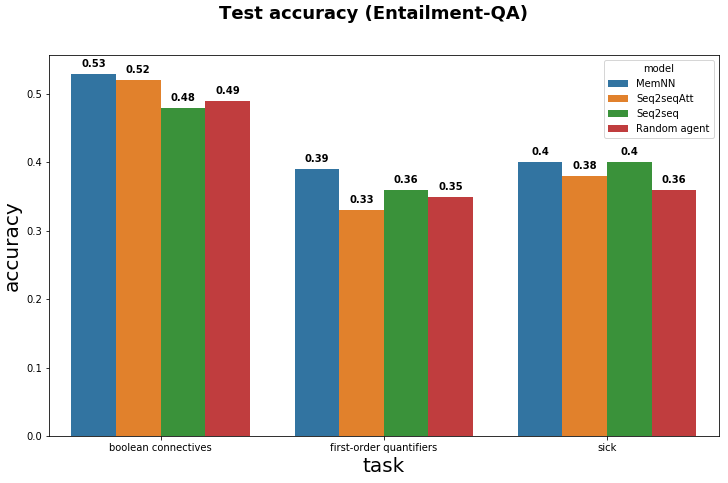
\includegraphics[scale=0.42]{images/comparative_results.png}
\end{center}
\end{frame}



\begin{frame}{Preliminary Results}
\begin{center}
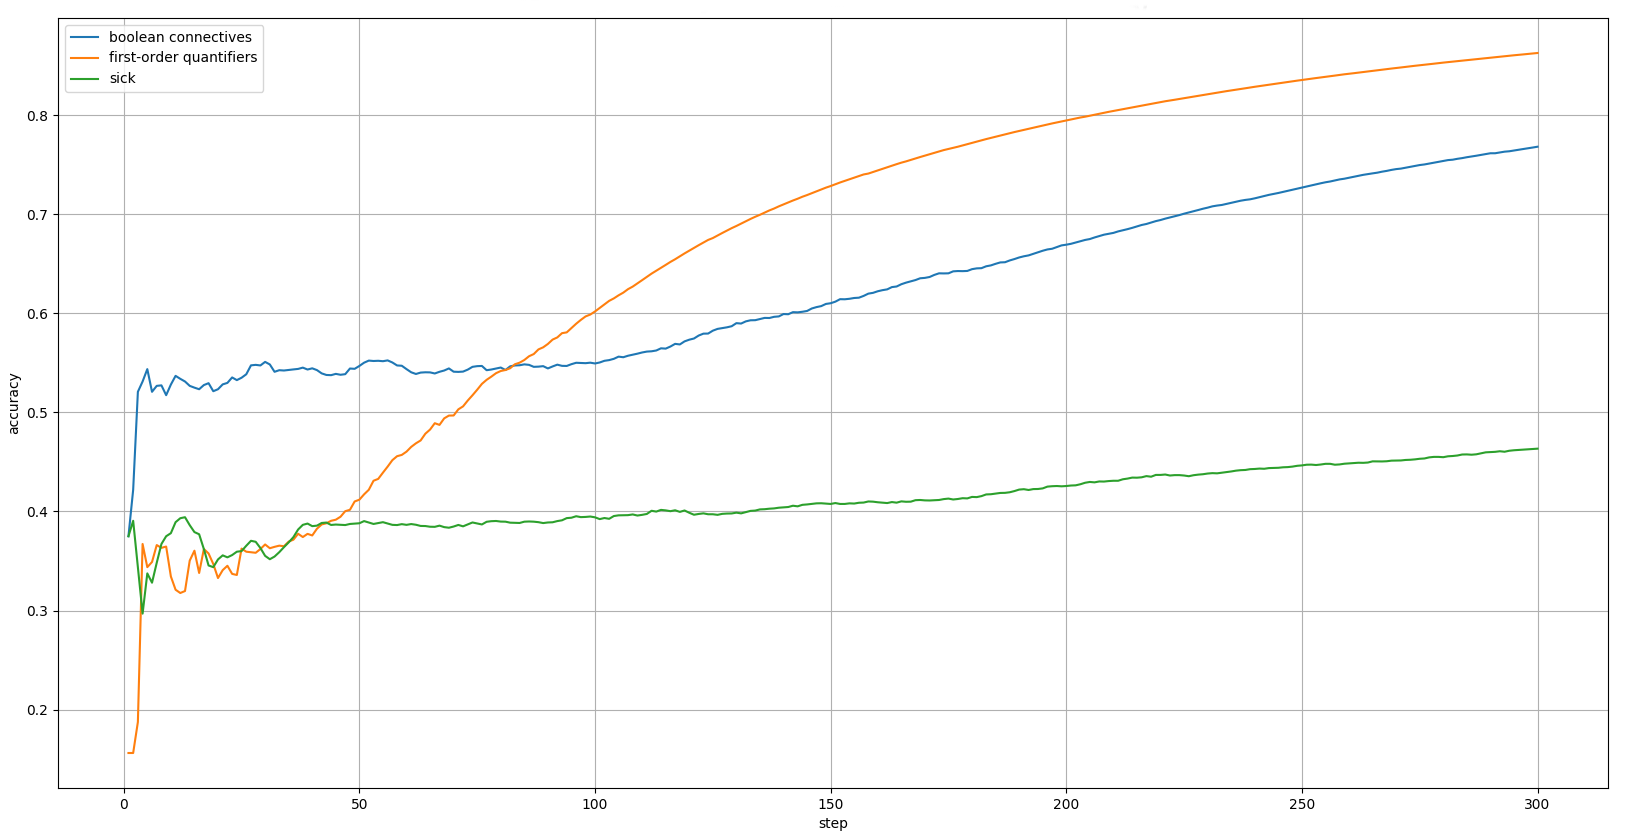
\includegraphics[scale=0.28]{images/training_acc_EntailQA_mem.png}
\end{center}
\end{frame}


\begin{frame}{Preliminary Results}
\begin{center}
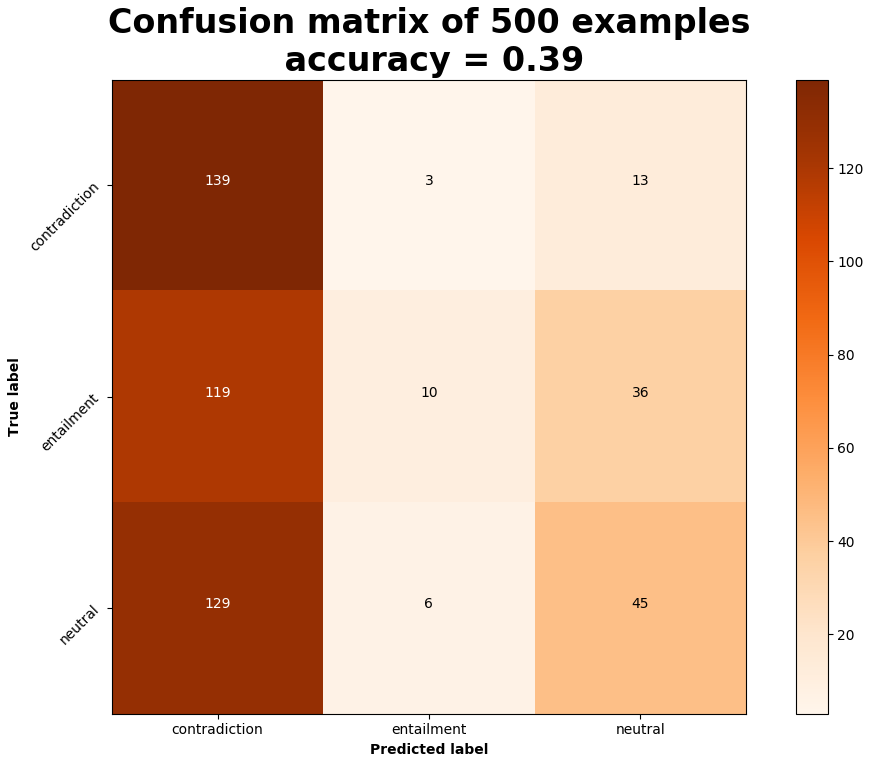
\includegraphics[scale=0.42]{images/cm_mem_EntailQA2.png}
\end{center}
\end{frame}


\begin{frame}{Future Steps}
\begin{itemize}
\item Apply regularization strategies on the available models to overcome the reported overfitting problem. 
\item Finish the Entailment-QA corpus to have a fine grain analysis of the result that we are seeing on the SICK corpus.
\item Explore the different extensions for all mentioned models.
\item Explore new models not mentioned here, like Dynamic Memory Networks \cite{KumarISBEPOGS15} and the models using the Memory Attention and Composition (MAC) cell \cite{Manning18}.
\item Create a visual version of the Entailment-QA to test logical inference with images.
\item There is a different literature that frames the dialog problem as an MDP (Markovian Decision Process) and a POMDP (Partially Observable Markovian Decision Process) applying different techniques of reinforcement learning (a recent example is \cite{Li:2016}). It is fruitful to investigate if these techniques can help our research.
\item One of the main focused here is model comparison. It would be fruitful if we could use the available literature  on the theory of comparing models (e.g., \cite{BenavoliCDZ17}) to refine our analysis.
\end{itemize}
\end{frame}


\begin{frame}{Schedule}
\begin{center}
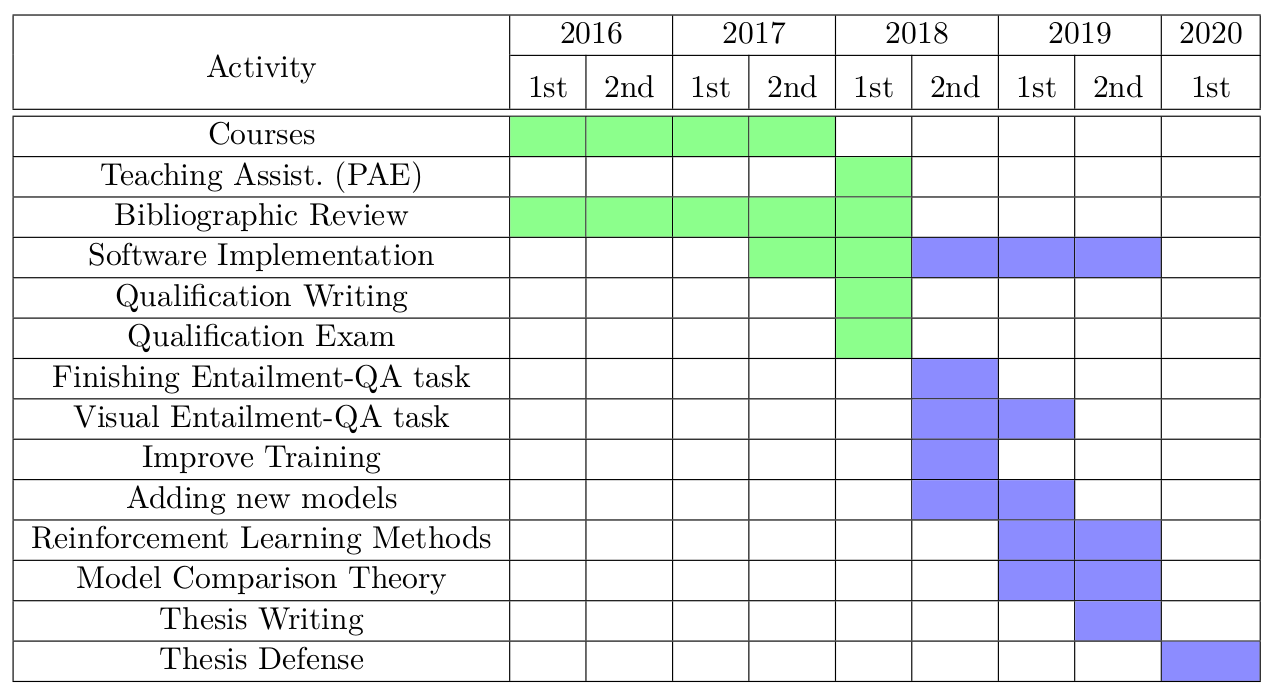
\includegraphics[scale=0.24]{images/workplan.png}
\end{center}
\end{frame}



\begin{frame}[allowframebreaks]{References}

  \bibliography{my_references}
  \bibliographystyle{abbrv}

\end{frame}

\end{document}




\end{document}